\documentclass[11pt]{article}


\usepackage{tkz-euclide}
%\usepackage{tkz-base}
%\usetikzlibrary{calc,patterns,angles,quotes,babel}
\usepackage{tkz-euclide}
\usepackage{pgfplots}
\usetkzobj{all}
\usetikzlibrary{shapes.geometric}
\usepackage{amssymb}

\usepgflibrary{arrows}
\usetikzlibrary{arrows} 
\pgfplotsset{compat=newest}
\begin{document}
%\section{Module 1: Elementaire rekenvaardigheden A}
\begin{center}
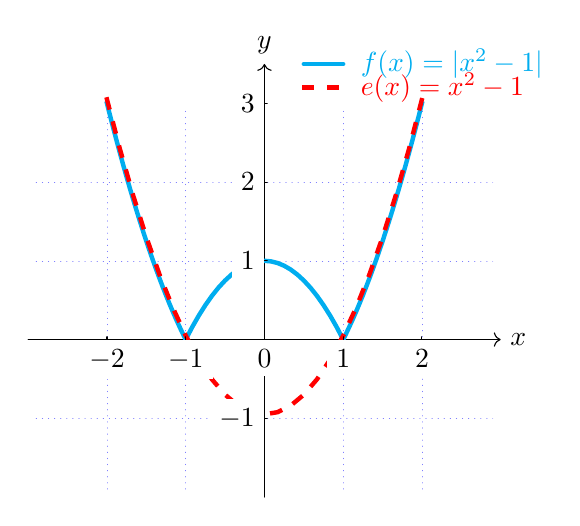
\begin{tikzpicture}[scale=1,cap=round]

% Styles
\tikzstyle{axes}=[]
\tikzstyle help lines=[color=blue!50,very thin,dotted]

% grid
\draw[style=help lines,step=1cm] (-2.9,-1.9) grid (2.9,2.9);


\draw[->] (-3,0) -- (3,0) node[right] {$x$};
\draw[->] (0,-2) -- (0,3.5) node[above] {$y$};

%\draw[fill,cyan](1,1)circle [radius=0.025];

\draw[cyan,cap=rect,ultra thick, domain=-2:-1] plot (\x, {\x*\x-1});

\draw[cyan,cap=rect,ultra thick, domain=-1:1] plot (\x, {-1*(\x*\x-1)});

\draw[cyan,cap=rect,ultra thick, domain=1:2] plot (\x, {\x*\x-1}) node[above, right]{};

\draw[red,cap=rect, loosely dashed, ultra thick, domain=-2:2] plot (\x, {(\x*\x-1)+0.05}) node[above,yshift=-.7cm, right]{};

%legende
\tkzDefPoint(0.5,3.5){A}
\tkzDefPoint(1,3.5){B}
\tkzLabelPoint[right,xshift=+0.1cm](B){${\color{cyan}f(x)=|x^2-1|}$}
\tkzDrawSegment[cyan,ultra thick](A,B)

\tkzDefPoint(0.5,3.2){C}
\tkzDefPoint(1,3.2){D}
\tkzLabelPoint[right,xshift=+0.1cm](D){${\color{red}e(x)=x^2-1}$}
\tkzDrawSegment[red,cap=rect, loosely dashed, ultra thick](C,D)



%getallen op de x-as en lijntjes   
\foreach \x/\xtext in {-2,-1,0, 1,2}
	\draw[xshift=\x cm] (0pt,1pt) -- (0pt,0pt) node[below,fill=white]
	{$\xtext$};,3
	
%getallen op de y-as en lijntjes  
%BEGIN LUS
\foreach \y/\ytext in {-1,1,2,3}
	\draw[yshift=\y cm] (1pt,0pt) -- (0pt,0pt) node[left,fill=white]
	{$\ytext$}; %EINDE LUS



\end{tikzpicture}
\end{center}

\input{1_elem_rekenvaardigheden_A/Fig_module_1_1_6_parRegelSom}
\begin{center}
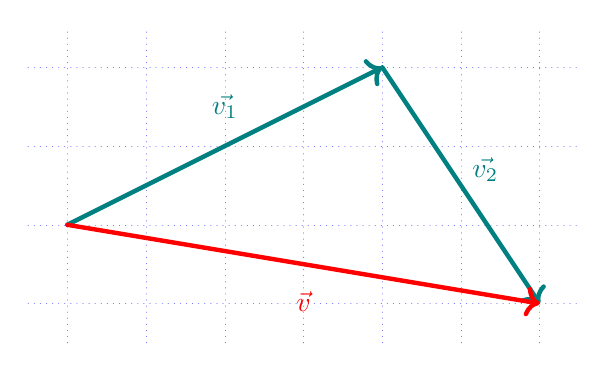
\begin{tikzpicture}[scale=1,cap=round]

% Styles
\tikzstyle{axes}=[]
\tikzstyle help lines=[color=blue!50,very thin,dotted]

% grid
\draw[style=help lines,step=1cm] (-.5,-1.5) grid (6.5,2.5);



\draw[->,teal,ultra thick] (0,0) -- (4,2) node[pos=0.5,above,yshift=+0.2cm] {${\Huge\vec{v_1}}$};
\draw[->,teal,ultra thick] (4,2) -- (6,-1) node[pos=0.5,above,right,yshift=+0.2cm] {$\vec{v_2}$};
\draw[->,red,ultra thick] (0,0) -- (6,-1) node[pos=0.5,below,yshift=-0.2cm] {$\vec{v}$};


\end{tikzpicture}
\end{center}


%\input{dimitri_oefent_tikz}
\begin{center}
\begin{tikzpicture}[scale=1,cap=round]


% Styles
\tikzstyle{axes}=[]
\tikzstyle help lines=[color=blue!50,very thin,dotted]

% grid
\draw[style=help lines,step=1cm] (-2.9,-2.9) grid (2.9,2.9);


\draw[->] (-3,0) -- (3,0) node[right] {$x$};
\draw[->] (0,-3) -- (0,3) node[above] {$y$};

\draw[thick, dashed, cyan,domain=-2:2] plot(\x, \x)  node[right]{$f(x)=x$};
%\draw[fill,cyan](1,1)circle [radius=0.025];

\tkzDefPoint(-2,-2){A}
\tkzDefPoint(-1,-1){B}
\tkzDefPoint(0,0){C}
\tkzDefPoint(1,1){D}
\tkzDefPoint(2,2){E}


\foreach \n in {A,B,C,D,E}
\node at (\n)[circle,cyan,fill,inner sep=1.5pt]{};

%getallen op de x-as en lijntjes   
\foreach \x/\xtext in {-3,-2,-1,0, 1,2,3}
	\draw[xshift=\x cm] (0pt,1pt) -- (0pt,0pt) node[below,fill=white]
	{$\xtext$};
	
%getallen op de y-as en lijntjes  
%BEGIN LUS
\foreach \y/\ytext in {-3,-2,-1,1,2}
	\draw[yshift=\y cm] (1pt,0pt) -- (0pt,0pt) node[left,fill=white]
	{$\ytext$}; %EINDE LUS
\end{tikzpicture}
\end{center}


\input{1_elem_rekenvaardigheden_A/Fig_module_1_2_9_logFunc1}

\begin{center}
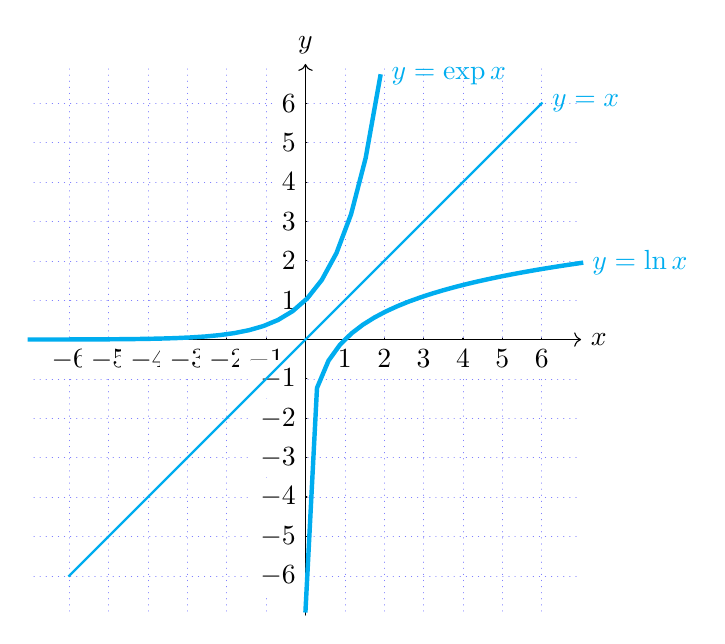
\begin{tikzpicture}[scale=0.5,cap=round]

% Styles
\tikzstyle{axes}=[]
\tikzstyle help lines=[color=blue!50,very thin,dotted]


%%%%%%%%%%%%%%%%%%%%%%%%%%%%%%%%
%		GRID
%%%%%%%%%%%%%%%%%%%%%%%%%%%%%%%%

\draw[style=help lines,step=1cm] (-6.9,-6.9) grid (6.9,6.9);

%%%%%%%%%%%%%%%%%%%%%%%%%%%%%%%%
%		ASSENSTELSEL
%%%%%%%%%%%%%%%%%%%%%%%%%%%%%%%%

\draw[->] (-7,0) -- (7,0) node[right] {$x$};
\draw[->] (0,-7) -- (0,7) node[above] {$y$};

%\draw[fill,cyan](1,1)circle [radius=0.025];

%\draw[red,cap=rect, loosely dashed, ultra thick, domain=-2:2] plot (\x, {(\x*\x-1)+0.05}) node[above,yshift=-.7cm, right]{};

%%%%%%%%%%%%%%%%%%%%%%%%%%%%%%%%
%legende
%%%%%%%%%%%%%%%%%%%%%%%%%%%%%%%%
%\tkzDefPoint(0.5,3.5){A}
%\tkzDefPoint(1,3.5){B}
%\tkzLabelPoint[right,xshift=+0.1cm](B){${\color{cyan}f(x)=|x^2-1|}$}
%\tkzDrawSegment[cyan,ultra thick](A,B)

%\tkzDefPoint(0.5,3.2){C}
%\tkzDefPoint(1,3.2){D}
%\tkzLabelPoint[right,xshift=+0.1cm](D){${\color{red}e(x)=x^2-1}$}
%\tkzDrawSegment[red,cap=rect, loosely dashed, ultra thick](C,D)


%%%%%%%%%%%%%%%%%%%%%%%%%%%%%%%%
%getallen op de x-as en lijntjes
%%%%%%%%%%%%%%%%%%%%%%%%%%%%%%%%   
\foreach \x/\xtext in {-6,-5,-4,-3,-2,-1,1,2,3,4,5,6}
	\draw[xshift=\x cm] (0pt,1pt) -- (0pt,0pt) node[below,fill=white]
	{$\xtext$};,3
	
%getallen op de y-as en lijntjes  
%BEGIN LUS
\foreach \y/\ytext in {-6,-5,-4,-3,-2,-1,1,2,3,4,5,6}
	\draw[yshift=\y cm] (1pt,0pt) -- (0pt,0pt) node[left,fill=white]
	{$\ytext$}; %EINDE LUS



%%%%%%%%%%%%%%%%%%%%%%%%%%%%%%%%
%		GRAFIEKEN
%%%%%%%%%%%%%%%%%%%%%%%%%%%%%%%%
\draw[cyan,cap=rect,thick, domain=-6:6] plot (\x, \x) node[above, right]{${\color{cyan}y=x}$};

\draw[cyan,cap=rect,ultra thick, domain=0.001:7] plot (\x, {ln{\x}}) node[above, right]{${\color{cyan}y=\ln{x}}$};

\draw[cyan,cap=rect,ultra thick, domain=-7:1.9] plot (\x, {exp{\x}}) node[above, right]{${\color{cyan}y=\exp{x}}$};


\end{tikzpicture}
\end{center}
\newpage
\section{Module 2: Elementaire rekenvaardigheden B}

%TODO polynoombenadering uitrekenen > zie cursus Algebra

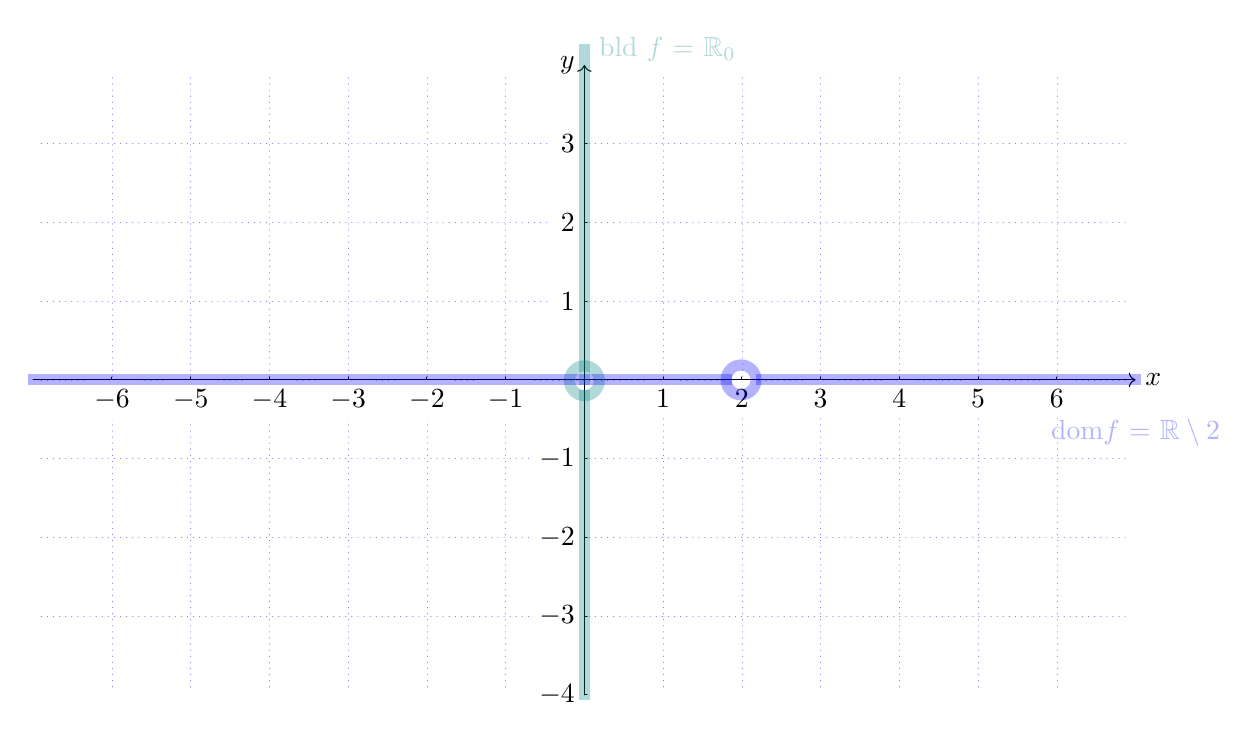
\begin{tikzpicture}[scale=1,cap=round]

% Styles
\tikzstyle{axes}=[]
\tikzstyle help lines=[color=blue!50,very thin,dotted]


%%%%%%%%%%%%%%%%%%%%%%%%%%%%%%%%
%		GRID
%%%%%%%%%%%%%%%%%%%%%%%%%%%%%%%%

\draw[style=help lines,step=1cm] (-6.9,-3.9) grid (6.9,3.9);



%%%%%%%%%%%%%%%%%%%%%%%%%%%%%%%%
%		ASSENSTELSEL
%%%%%%%%%%%%%%%%%%%%%%%%%%%%%%%%

\draw[->] (-7,0) -- (7,0) node[right] {$x$};
\draw[->] (0,-4) -- (0,4) node[left]{$y$};

%\draw[fill,cyan](1,1)circle [radius=0.025];

%\draw[red,cap=rect, loosely dashed, ultra thick, domain=-2:2] plot (\x, {(\x*\x-1)+0.05}) node[above,yshift=-.7cm, right]{};

%%%%%%%%%%%%%%%%%%%%%%%%%%%%%%%%
%legende
%%%%%%%%%%%%%%%%%%%%%%%%%%%%%%%%
%\tkzDefPoint(0.5,3.5){A}
%\tkzDefPoint(1,3.5){B}
%\tkzLabelPoint[right,xshift=+0.1cm](B){${\color{cyan}f(x)=|x^2-1|}$}
%\tkzDrawSegment[cyan,ultra thick](A,B)

%\tkzDefPoint(0.5,3.2){C}
%\tkzDefPoint(1,3.2){D}
%\tkzLabelPoint[right,xshift=+0.1cm](D){${\color{red}e(x)=x^2-1}$}
%\tkzDrawSegment[red,cap=rect, loosely dashed, ultra thick](C,D)


%%%%%%%%%%%%%%%%%%%%%%%%%%%%%%%%
%getallen op de x-as en lijntjes
%%%%%%%%%%%%%%%%%%%%%%%%%%%%%%%%   
\foreach \x/\xtext in {-6,-5,-4,-3,-2,-1,1,2,3,4,5,6}
	\draw[xshift=\x cm] (0pt,1pt) -- (0pt,0pt) node[below,fill=white]
	{$\xtext$};,3
	
%getallen op de y-as en lijntjes  
%BEGIN LUS
\foreach \y/\ytext in {-4,-3,-2,-1,1,2,3}
	\draw[yshift=\y cm] (1pt,0pt) -- (0pt,0pt) node[left,fill=white]
	{$\ytext$}; %EINDE LUS



%%%%%%%%%%%%%%%%%%%%%%%%%%%%%%%%
%		GRAFIEKEN
%%%%%%%%%%%%%%%%%%%%%%%%%%%%%%%%
%\draw[cyan,cap=rect,thick, domain=-6:6] plot (\x, \x) node[above, right]{${\color{cyan}y=x}$};v

%\draw[cyan,cap=rect,ultra thick, domain=-6:1.75] plot (\x, {(\x-2)^(-1)}) node[above,right]{};


%\draw[cyan,cap=rect,ultra thick, domain=2.25:6] plot (\x, {(\x-2)^(-1)}) node[above,yshift=+0.5cm,left]{$\color{cyan} y=\frac{1}{x-2}$};


%\draw[cyan,cap=rect,ultra thick, domain=-7:1.9] plot (\x, {exp{\x}}) node[above, right]{${\color{cyan}y=\exp{x}}$};

%%%%%%%%%%%%%%%%%%%%%%%%%%%%%%%%
%		MARKERINGEN
%%%%%%%%%%%%%%%%%%%%%%%%%%%%%%%%
%verticale lijn
\draw[-o,line width=4,teal, cap=rect,opacity=0.3] (0,-4) -- (0,0.25) node[right] {};
\draw[line width=4,teal, cap=rect,opacity=0.3] (0,0) -- (0,4.2) node[right] {bld $f$ = $\mathbb{R}_0$};
%horizontale lijn
\draw[arrows=-o,line width=4,blue, cap=rect,opacity=0.3] (-7,0) -- (2.25,0) node[right] {};
\draw[line width=4,blue, cap=rect,opacity=0.3] (2.25,0) -- (7,0) node[below,yshift=-0.3cm] {dom$f$ = $\mathbb{R}  \setminus 2 $};
 
\end{tikzpicture}

\input{2_elem_rekenvaardigheden_B/Fig_module_2_1_2_reele_functies_vb2}

\begin{center}
\begin{tikzpicture}[scale=1,cap=round]

% Styles
\tikzstyle{axes}=[]
\tikzstyle help lines=[color=blue!50,very thin,dotted]


%%%%%%%%%%%%%%%%%%%%%%%%%%%%%%%%
%		GRID
%%%%%%%%%%%%%%%%%%%%%%%%%%%%%%%%

\draw[style=help lines,step=1cm] (-3.9,-5.9) grid (3.9,5.9);



%%%%%%%%%%%%%%%%%%%%%%%%%%%%%%%%
%		ASSENSTELSEL
%%%%%%%%%%%%%%%%%%%%%%%%%%%%%%%%

\draw[->] (-5,0) -- (7,0) node[right] {$x$};
\draw[->] (0,-7) -- (0,7) node[left]{$y$};

%\draw[fill,cyan](1,1)circle [radius=0.025];

%\draw[red,cap=rect, loosely dashed, ultra thick, domain=-2:2] plot (\x, {(\x*\x-1)+0.05}) node[above,yshift=-.7cm, right]{};

%%%%%%%%%%%%%%%%%%%%%%%%%%%%%%%%
%legende
%%%%%%%%%%%%%%%%%%%%%%%%%%%%%%%%
%\tkzDefPoint(0.5,3.5){A}
%\tkzDefPoint(1,3.5){B}
%\tkzLabelPoint[right,xshift=+0.1cm](B){${\color{cyan}f(x)=|x^2-1|}$}
%\tkzDrawSegment[cyan,ultra thick](A,B)

%\tkzDefPoint(0.5,3.2){C}
%\tkzDefPoint(1,3.2){D}
%\tkzLabelPoint[right,xshift=+0.1cm](D){${\color{red}e(x)=x^2-1}$}
%\tkzDrawSegment[red,cap=rect, loosely dashed, ultra thick](C,D)


%%%%%%%%%%%%%%%%%%%%%%%%%%%%%%%%
%getallen op de x-as en lijntjes
%%%%%%%%%%%%%%%%%%%%%%%%%%%%%%%%   
\foreach \x/\xtext in {-4,-3,-2,-1,1,2,3,4}
	\draw[xshift=\x cm] (0pt,1pt) -- (0pt,0pt) node[below,fill=white]
	{$\xtext$};,3
	
%getallen op de y-as en lijntjes  
%BEGIN LUS
\foreach \y/\ytext in {-6,-5,-4,-3,-2,-1,1,2,3,4,5,6}
	\draw[yshift=\y cm] (1pt,0pt) -- (0pt,0pt) node[left,fill=white]
	{$\ytext$}; %EINDE LUS



%%%%%%%%%%%%%%%%%%%%%%%%%%%%%%%%
%		GRAFIEKEN
%%%%%%%%%%%%%%%%%%%%%%%%%%%%%%%%
%\draw[cyan,cap=rect,thick, domain=-6:6] plot (\x, \x) node[above, right]{${\color{cyan}y=x}$};

\draw[cyan,cap=rect,ultra thick, domain=-1.2:3.5] plot (\x, {
	pow(\x,3)-3*pow(\x,2)		% <- plaats het functievoorschrift hier
}) node[above]{$f(x)=x^3-3x^2$};

 
%node[blue]{stijgen} 
%\draw[cyan,cap=rect,ultra thick, domain=2.25:6] plot (\x, {(\x-2)^(-1)}) node[above,yshift=+0.5cm,left]{$\color{cyan} y=\frac{1}{x-2}$};


%\draw[cyan,cap=rect,ultra thick, domain=-7:1.9] plot (\x, {exp{\x}}) node[above, right]{${\color{cyan}y=\exp{x}}$};

%%%%%%%%%%%%%%%%%%%%%%%%%%%%%%%%
%		MARKERINGEN
%%%%%%%%%%%%%%%%%%%%%%%%%%%%%%%%
%verticale lijn
%\draw[-o,line width=4,teal, cap=rect,opacity=0.3] (0,-4) -- (0,0.25) node[right] {};
%\draw[line width=4,teal, cap=rect,opacity=0.3] (0,0) -- (0,4.2) node[right] {bld $f$ = $\mathbb{R}_0$};
%horizontale lijn

 \draw[white,fill=blue,opacity=.5] (1,-2) circle [radius=.1]   node[blue, above,xshift=-1.1cm,opacity=1] {buigpunt in $(1,-2)$};


 
\draw[teal,cap=rect,line width=4, opacity=.5, domain=.5:1.5] plot (\x, {
	-2-3*(\x-1)		% <- plaats het functievoorschrift hier
}) node[opacity=1,above]{};


\draw[] (1.5,1.5) node[blue] {hol of concaaf};
\draw[] (1.5,-5) node[blue] {bol of convex};

\end{tikzpicture}
\end{center}

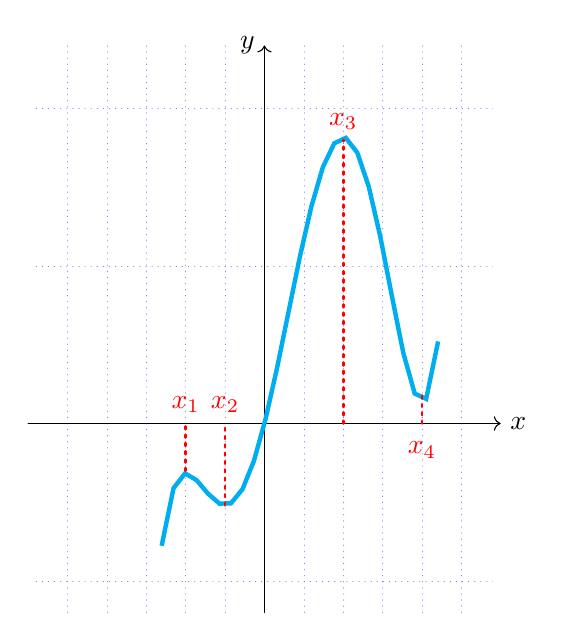
\begin{tikzpicture}[xscale=1,yscale=4,cap=round]

% Styles
\tikzstyle{axes}=[]
\tikzstyle help lines=[color=blue!50,very thin,dotted]

%%%%%%%%%%%%%%%%%%%%%%%%%%%%%%%%
%		GRID
%%%%%%%%%%%%%%%%%%%%%%%%%%%%%%%%

\draw[style=help lines,step=0.5cm] (-2.9,-0.6) grid (2.9,1.2);

%%%%%%%%%%%%%%%%%%%%%%%%%%%%%%%%
%		ASSENSTELSEL
%%%%%%%%%%%%%%%%%%%%%%%%%%%%%%%%

\draw[->] (-3,0) -- (3,0) node[right] {$x$};
\draw[->] (0,-0.6) -- (0,1.2) node[left]{$y$};

%\draw[fill,cyan](1,1)circle [radius=0.025];
%\draw[red,cap=rect, loosely dashed, ultra thick, domain=-2:2] plot (\x, {(\x*\x-1)+0.05}) node[above,yshift=-.7cm, right]{};

%%%%%%%%%%%%%%%%%%%%%%%%%%%%%%%%
%legende
%%%%%%%%%%%%%%%%%%%%%%%%%%%%%%%%
%\tkzDefPoint(0.5,3.5){A}
%\tkzDefPoint(1,3.5){B}
%\tkzLabelPoint[right,xshift=+0.1cm](B){${\color{cyan}f(x)=|x^2-1|}$}
%\tkzDrawSegment[cyan,ultra thick](A,B)

%\tkzDefPoint(0.5,3.2){C}
%\tkzDefPoint(1,3.2){D}
%\tkzLabelPoint[right,xshift=+0.1cm](D){${\color{red}e(x)=x^2-1}$}
%\tkzDrawSegment[red,cap=rect, loosely dashed, ultra thick](C,D)


%%%%%%%%%%%%%%%%%%%%%%%%%%%%%%%%
%getallen op de x-as en lijntjes
%%%%%%%%%%%%%%%%%%%%%%%%%%%%%%%%   
%\foreach \x/\xtext in {-2,-1,1,2}
%	\draw[xshift=\x cm] (0pt,1pt) -- (0pt,0pt) node[below,fill=white]
%	{$\xtext$};,3
	
%getallen op de y-as en lijntjes  
%BEGIN LUS
%\foreach \y/\ytext in {-1,1}
%	\draw[yshift=\y cm] (1pt,0pt) -- (0pt,0pt) node[left,fill=white]
%	{$\ytext$}; %EINDE LUS



%%%%%%%%%%%%%%%%%%%%%%%%%%%%%%%%
%		GRAFIEKEN
%%%%%%%%%%%%%%%%%%%%%%%%%%%%%%%%
%1.926583164702752926
%0.6148052613028164304
%%-14.35341068538563647
%-59.14215224350418509
%104.9541745028843565
%191

\draw[cyan,cap=rect,ultra thick, domain=-1.3:2.2] plot (\x, {
0.2*pow(\x,5)-(3/8)*pow(\x,4)-(2/3)*pow(\x,3)+(3/4)*pow(\x,2)+\x 	
%	*(	(\x+2)*(\x+1)*(\x+0.5)*(\x-1)*(\x-2) ) *0.2
	%pow(\x,5)+0.5*pow(\x,4)-5*pow(\x,3)+3*pow(\x,1)-1 )*.1 
	% <- plaats het functievoorschrift hier
}) node[above, yshift=+0.5cm,xshift=+1.3cm]{$$};
%f(x)=x^5+\frac{1}{2}x^4-5x^3-\frac{5}{2}x^2+4x-2

 
%node[blue]{stijgen} 
%\draw[cyan,cap=rect,ultra thick, domain=2.25:6] plot (\x, {(\x-2)^(-1)}) node[above,yshift=+0.5cm,left]{$\color{cyan} y=\frac{1}{x-2}$};


%\draw[cyan,cap=rect,ultra thick, domain=-7:1.9] plot (\x, {exp{\x}}) node[above, right]{${\color{cyan}y=\exp{x}}$};

%%%%%%%%%%%%%%%%%%%%%%%%%%%%%%%%
%		MARKERINGEN
%%%%%%%%%%%%%%%%%%%%%%%%%%%%%%%%
%verticale lijn
\draw[line width=1,red, dotted, opacity=1] (-1,-.15) -- (-1,0) node[above] {$x_1$};
\draw[line width=1,red, dotted, opacity=1] (-0.5,-.26) -- (-0.5,0) node[above] {$x_2$};
\draw[line width=1,red,opacity=1,dotted] (1,0) -- (1,0.9) node[above] {$x_3$};
\draw[line width=1,red,opacity=1,dotted] (2,0) -- (2,0.1) node[below,yshift=-.5cm] {$x_4$};
%\draw[line width=4,teal, cap=rect,opacity=0.3] (0,0) -- (0,4.2) node[right] {bld $f$ = $\mathbb{R}_0$};
%horizontale lijn

% \draw[white,fill=blue,opacity=.5] (1,-2) circle [radius=.1]   node[blue, above,xshift=-1.1cm,opacity=1] {buigpunt in $(1,-2)$};


 
%\draw[teal,cap=rect,line width=4, opacity=.5, domain=.5:1.5] plot (\x, {
%	-2-3*(\x-1)		% <- plaats het functievoorschrift hier
%}) node[opacity=1,above]{};


%\draw[] (1.5,1.5) node[blue] {hol of concaaf};
%\draw[] (1.5,-5) node[blue] {bol of convex};

\end{tikzpicture}
 
\input{2_elem_rekenvaardigheden_B/Fig_module_2_1_2_verloop_vb2}
\input{2_elem_rekenvaardigheden_B/Fig_module_2_1_2_verloop_vb3}
%TODO waarom verschijnt dat hier niet? 


\end{document}